\chapter{Metodologia}

Este capítulo aborda o planejamento e execução do projeto, contendo os procedimentos e técnicas utilizadas, possibilitando a sua  replicação.

Tendo em vista os conceitos descritos nos capítulos anteriores, o presente trabalho tem como objetivo responder à seguinte questão problema:

\begin{center}
\textit{É possível extrair o perfil temático dos deputados através da análise dos seus discursos e proposições utilizando técnicas de aprendizado de máquina e processamento de linguagem natural?}
\end{center}

Além disso, será construído um \textit{website} com o intuito de fornecer uma forma melhor de visualização dos dados obtidos na análise dos discursos e proposições, através de gráficos interativos que garantam que o usuário tenha uma boa experiência ao utilizá-lo.

\section{Trabalhos Relacionados}

Durante a pesquisa bibliográfica realizada neste trabalho, encontrou-se alguns trabalhos que também fizeram análise de textos parlamentares utilizando aprendizado bayesiano. O Retórica Parlamentar\footnote{http://retorica.labhackercd.net/about.html}, idealizado por Davi Moreira\footnote{https://github.com/davi-moreira}, Manoel Galdino\footnote{https://github.com/mgaldino} e Luis Carli\footnote{https://github.com/luiscarli}, utiliza os discursos proferidos pelos parlamentares no Pequeno Expediente e no Grande Expediente da Câmara dos Deputados para promover a transparência do mandato e fornecer subsídios para o controle social com a divulgação dos temas mais debatidos em Plenário.

A técnica utilizada pelo Retórica para a classificação dos discursos é um modelo bayesiano hierárquico, descrito por \citeonline{grimmer2009}, onde através de aprendizado não supervisionado são gerados \(k\) \textit{clusters}, sendo \(k\) um valor escolhido ao executar o algoritmo. O resultado é exportado para o formato \textit{csv} e contém os termos mais frequentes de cada cluster. Em seguida, um especialista deve ler e rotular cada \textit{cluster}.

A visualização dos dados é feita através de um gráfico de bolhas, em que cada bolha representa a relevância (medida pela frequência) de cada tema dentre todos os deputados analisados. Dentro de cada bolha são colocados os deputados que enfatizam aquele tema nos seus discursos. Um deputado está associado a um único tema, que é o tema mais enfatizado por ele nos seus discursos.

\begin{figure}[h]
    \centering
    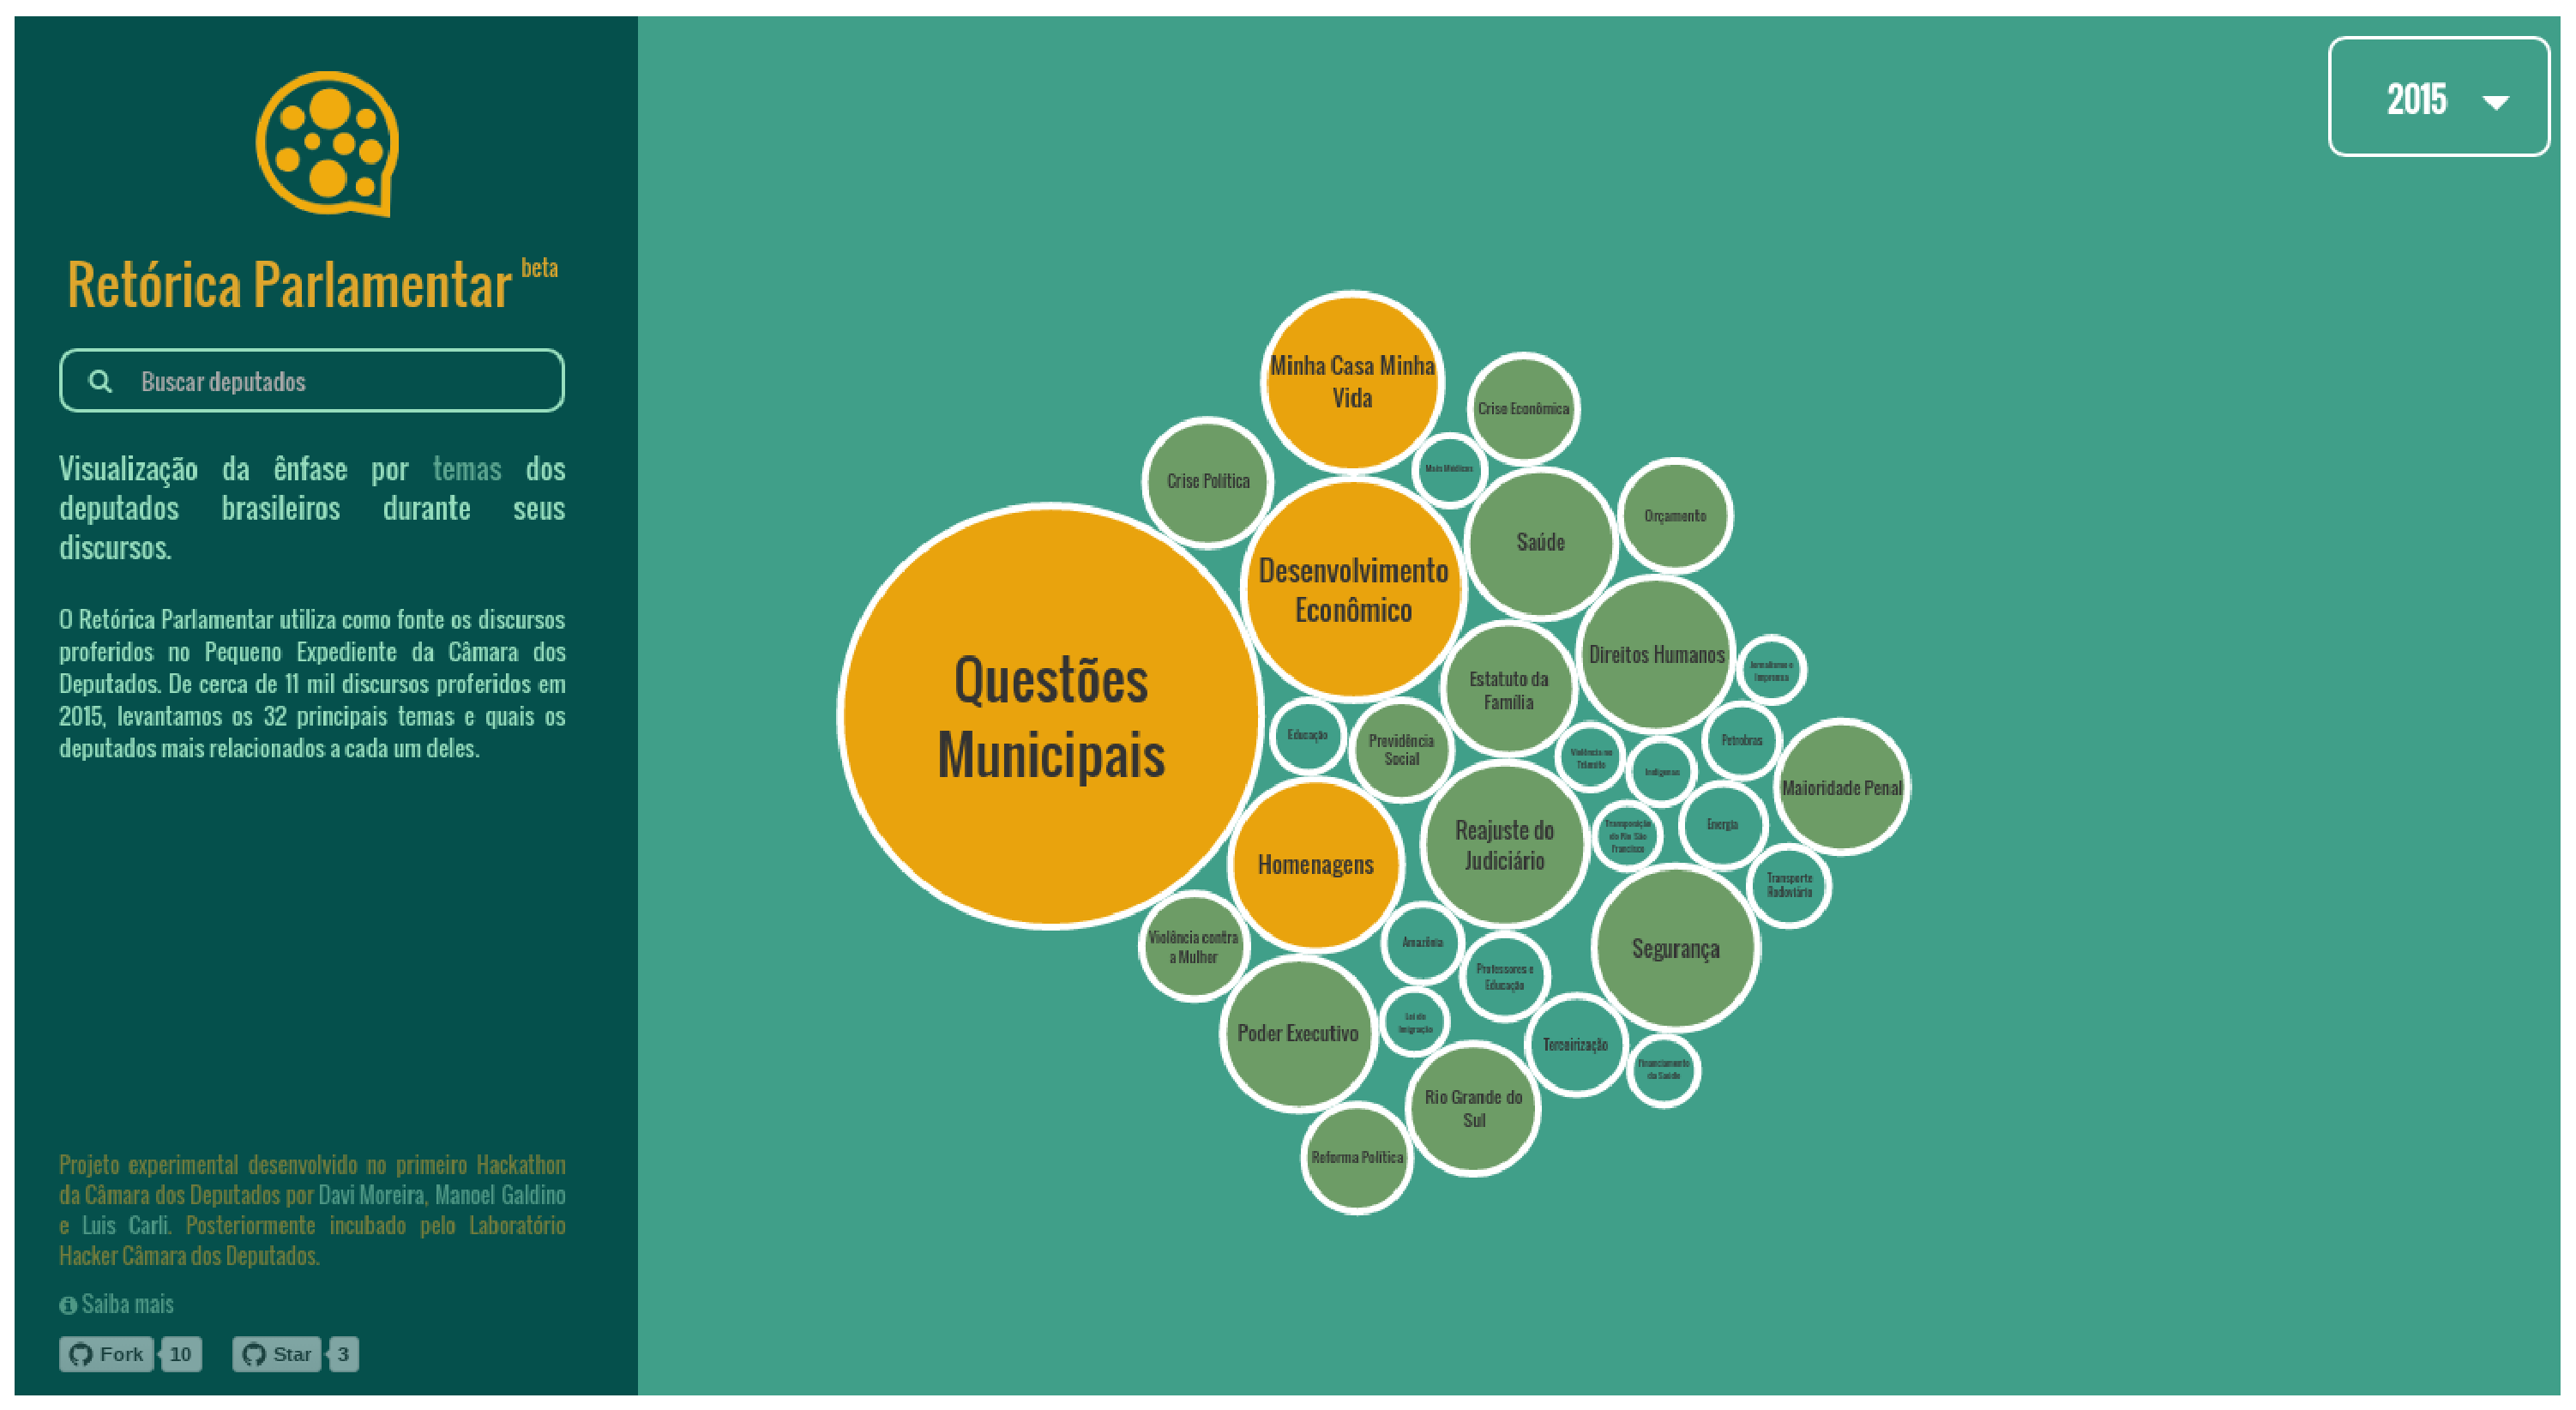
\includegraphics[scale=0.3]{figuras/retorica.eps}
    \caption{Retórica Parlamentar}
\end{figure}

\section{Obtenção dos Dados}
\label{obtencao-dados}

Todos os dados utilizados para análise foram obtidos através do portal de dados abertos da Câmara dos Deputados\footnote{http://www.camara.leg.br/transparencia/dados-abertos}, que é dividido em duas partes: dados legislativos e dados referentes à cota parlamentar, que não foram utilizados nesse trabalho. Os dados legislativos estão relacionados à informações sobre deputados, órgãos legislativos, proposições, sessões plenárias e reuniões de comissões.

\subsection{\textit{Webservice} da Câmara dos Deputados}

Atualmente, o \textit{Webservice} da Câmara dos Deputados é estruturado de acordo com os padrões \textit{SOAP} (\textit{Simple Object Access Protocol}, em português Protocolo Simples de Acesso a Objetos), que se baseiam na linguagem de marcação \textit{XML} e utilizam, principalmente, chamada de procedimento remoto (\textit{RPC}) e protocolo de transferência de hipertexto (\textit{HTTP}) para a transmissão das mensagens \cite{soap2007}.


No entanto, o \textit{webservice} possui alguns aspectos que podem ser melhorados. Como os dados são fornecidos utilizando o formato \textit{XML}, eles não são ``tipados'', ou seja, independente do tipo (inteiro, data, texto, etc) eles são representados com \textit{strings}. Alguns dados são ambíguos, como os referentes aos deputados, onde existem ``ideCadastro'' e ``idParlamentar'', que são utilizados como parâmetros de entrada de requisições distintas. Outro problema é que requisições comuns precisam ser feitas indiretamente pois não agrega conteúdos com \textit{queries} relacionais, como normalmente são as \textit{API REST}. Além disso, o inteiro teor dos discursos parlamentares estão disponíveis apenas em formato \textit{RTF}, o que dificulta um pouco a utilização dos mesmos.

No momento de escrita desse trabalho, se encontra em desenvolvimento uma nova versão do portal de dados abertos da Câmara dos Deputados, que está em fase de testes e já pode ser acessada pela sociedade\footnote{https://dadosabertos.camara.leg.br/}, porém ainda não possui os mesmos dados disponíveis na versão anterior. O novo \textit{webservice} segue os padrões REST e possibilita a escolha do formato de retorno, podendo ser em \textit{XML} ou em  \textit{JSON}. Além disso, visa corrigir os problemas encontrados na versão anterior (alguns mencionados no parágrafo acima), bem como aumentar a quantidade de dados disponíveis. Uma das promessas é disponibilizar o texto completo das proposições, que hoje só é disponível via \textit{PDF} sendo que alguns são apenas imagens \textit{scaneadas} dos documentos físicos.

A estrutura do \textit{webservice} da Câmara dos Deputados pode ser encontrada no apêndice \ref{estrutura-webservice}

\section{Proposta de Desenvolvimento}

\subsection{\textit{Pygov-br}}

\textit{Pygov-br} é uma biblioteca \textit{python} desenvolvida no contexto desse trabalho cujo objetivo é centralizar o consumo de \textit{APIs} e \textit{webservices} governamentais brasileiros. Além dos dados, a biblioteca também irá fornecer um conjunto de \textit{plugins} para os principais \textit{frameworks} para desenvolvimento \textit{web}, para facilitar a utilização dos dados abertos, bem como o cruzamento de dados provenientes de diferentes órgãos governamentais.

Atualmente, a biblioteca oferece suporte somente ao \textit{webservice} da Câmara dos Deputados, tanto para o consumo dos dados quanto para o uso em aplicações \textit{Django}, já que para o desenvolvimento do presente trabalho apenas esses dados seriam utilizados.

A estrutura para o consumo dos \textit{webservices} não é fixa, pois cada \textit{webservice} possui suas características. A implementação para consumir os dados da Câmara dos Deputados segue a estrutura do \textit{webservice} (figura \ref{estrutua_camara_deputados}), com algumas alterações. Além disso, todos o código implementado foi escrito em inglês, apesar dos dados estarem em português.

\begin{figure}[h]
    \centering
    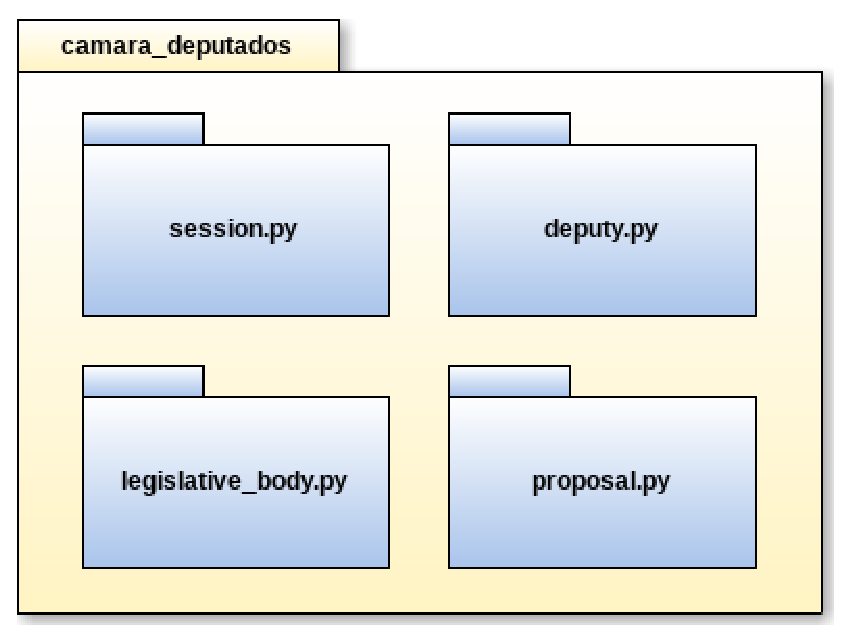
\includegraphics[scale=0.5]{figuras/camara_deputados.eps}
    \caption{Estrutura do módulo de consumo de dados da Câmara dos Deputados}
    \label{estrutua_camara_deputados}
\end{figure}


Como dito anteriormente, a \textit{pygov-br} também possui módulos para utilização em conjunto com os \textit{frameworks} de desenvolvimento \textit{web} mais utilizados na comunidade. Porém, como a solução \textit{web} desenvolvida nesse trabalho utilizará o \textit{framework Django}, a atual implementação da \textit{pygov-br} possui suporte somente a esse \textit{framework}.

O módulo \textbf{django\_apps} contém os \textit{plugins} para utilização em projetos \textit{Django}. Esses \textit{apps} possuem apenas as \textit{models} (na linguagem da arquitetura \textit{MVT} do \textit{Django}) já que o objetivo é somente facilitar a permanência das informações obtidas dos \textit{webservices} governamentais em um banco de dados. No caso da Câmara dos Deputados, os dados utilizados nesse trabalho ficam disponíveis seguindo o modelo entidade-relacionamento na figura \ref{modelo-eer}. Podemos notar que todas as colunas de todas as tabelas se encontram em em inglês, por motivos de padronização do código.

Após a apresentação da primeira parte desse trabalho, foram realizadas algumas sugestões quanto à tradução dos termos para o inglês. Entretanto, como estava prevista uma nova API da Câmara dos Deputados com alterações significativas que implicariam em uma reescrita considerável do código da \textit{pygov-br}, ficou decidido que essas alterações de nomenclaturas seriam realizadas no momento de reescrita da biblioteca.


\begin{figure}[h]
    \centering
    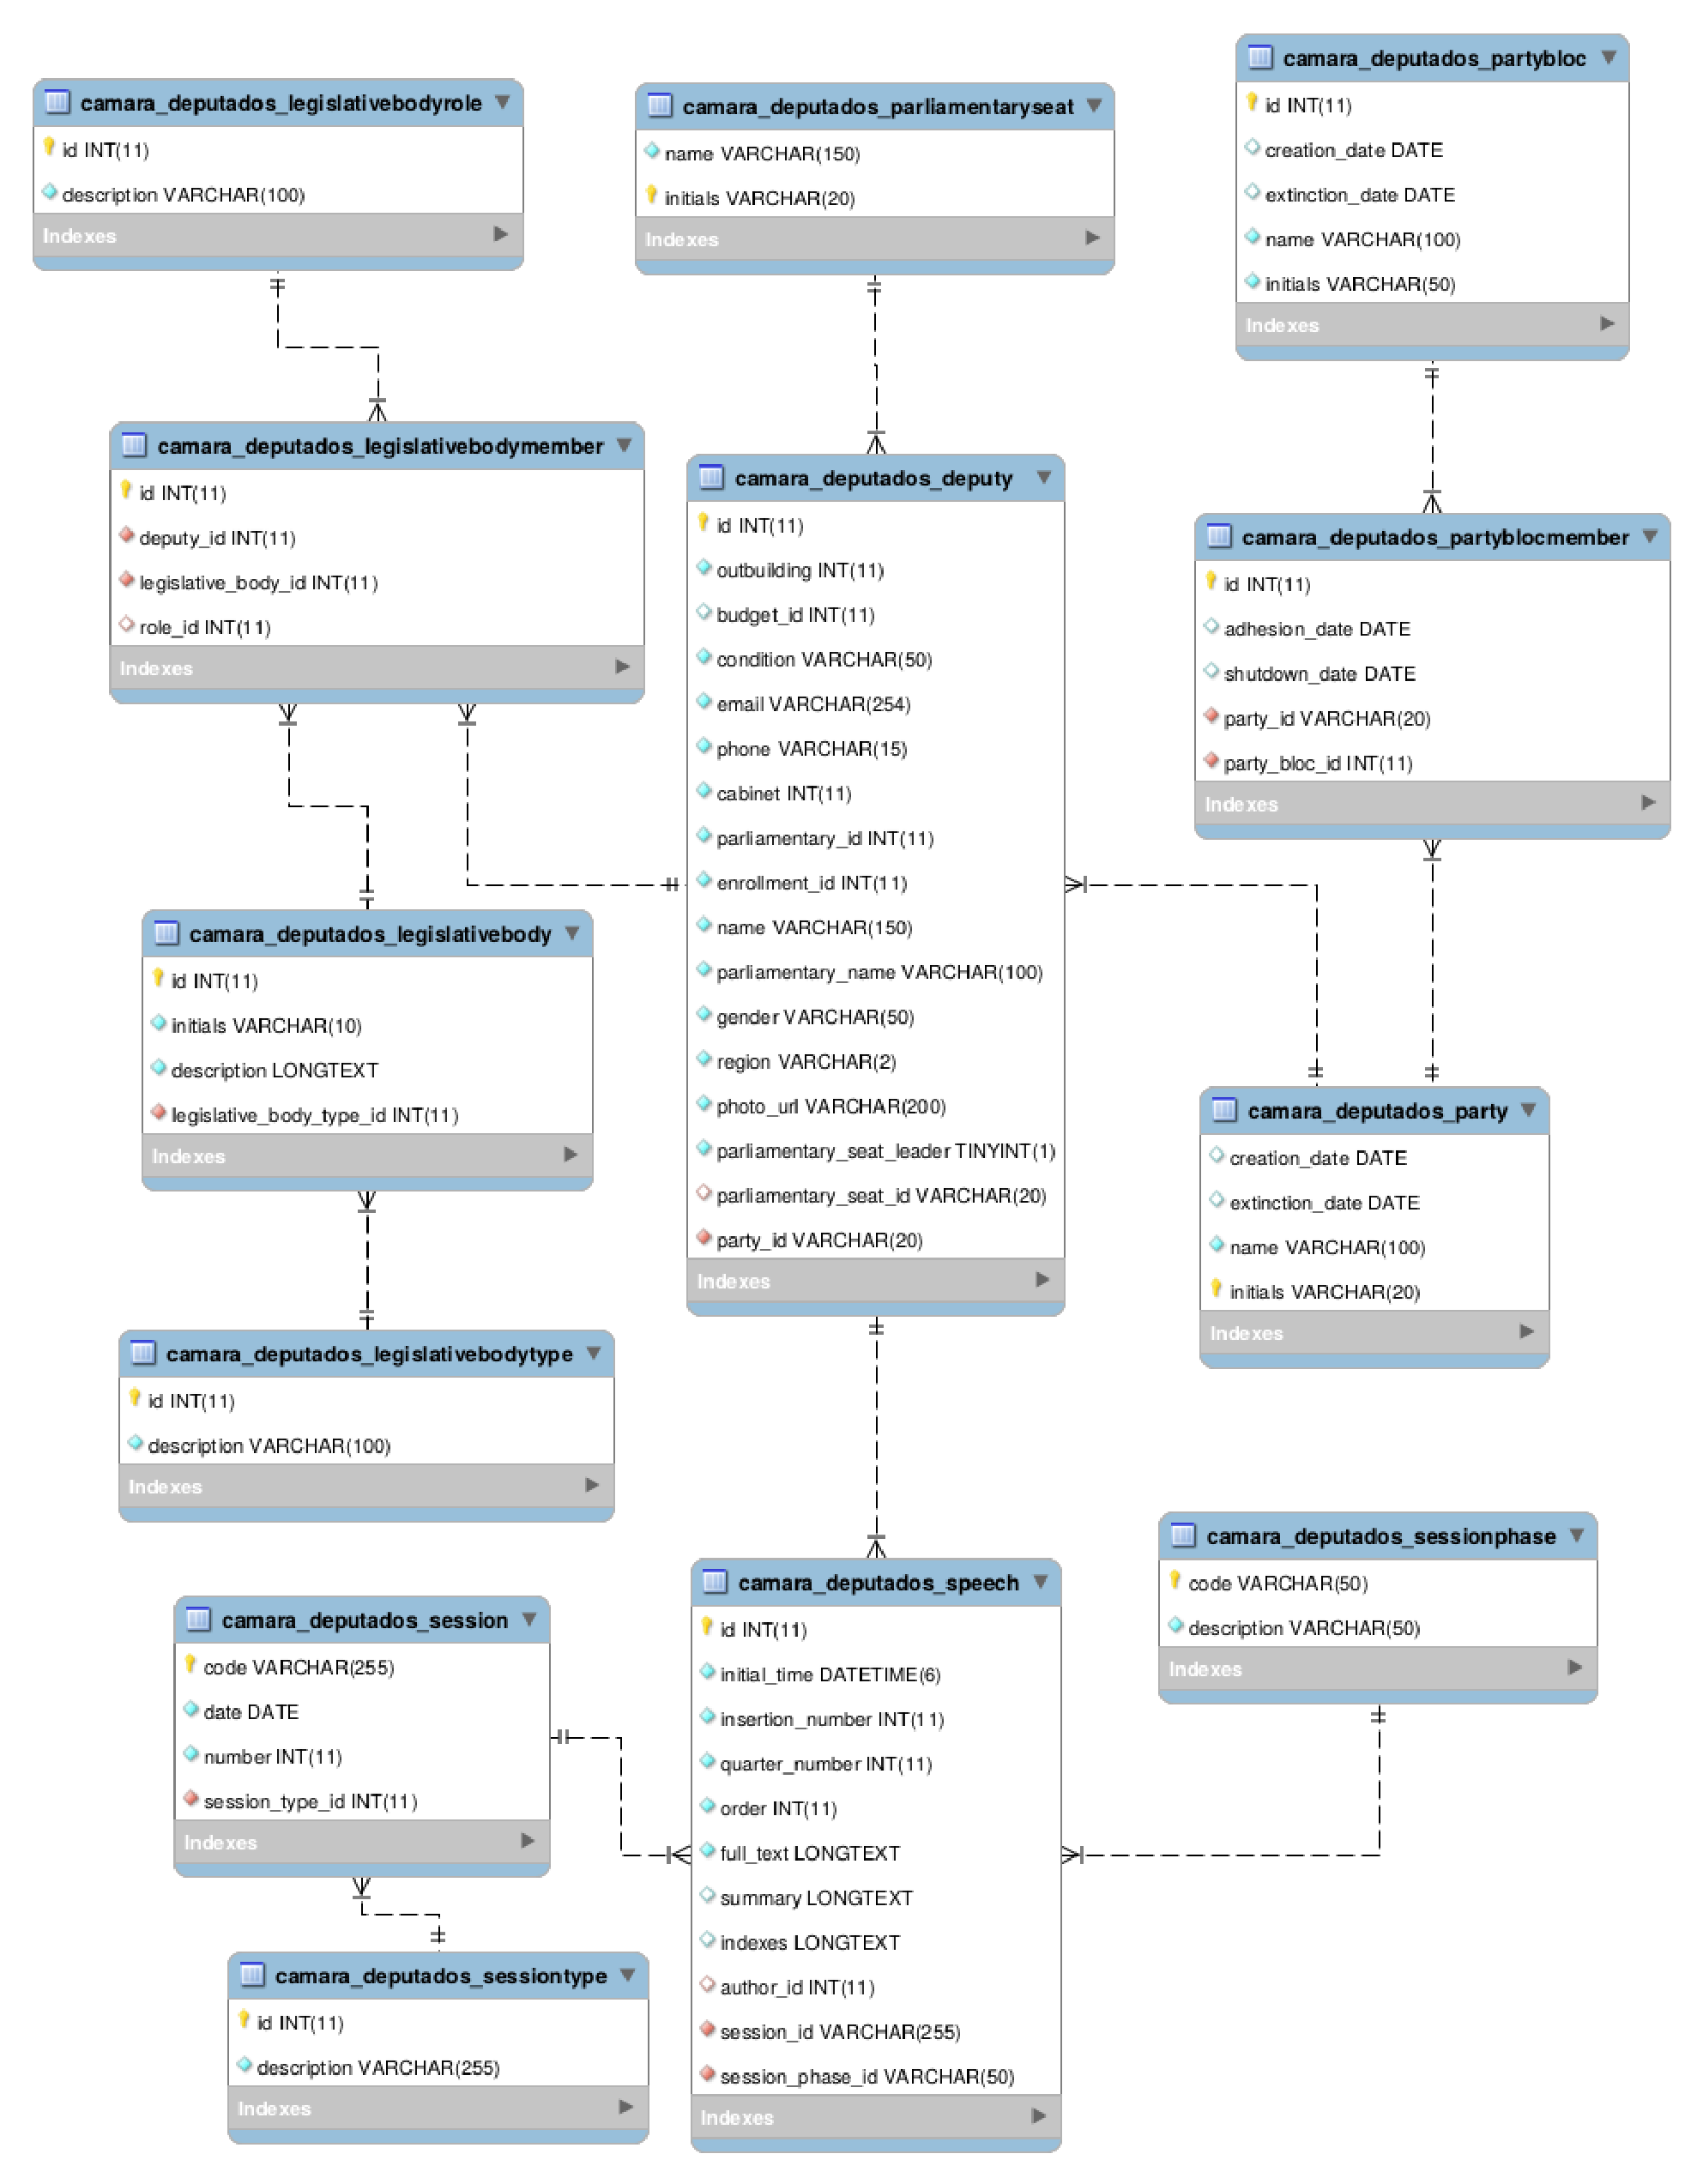
\includegraphics[scale=0.5]{figuras/pygov-eer.eps}
    \caption{Modelo entidade-relacionamento do banco de dados utilizado}
    \label{modelo-eer}
\end{figure}

\clearpage

\subsection{Tenho Dito}

``Tenho Dito'' é uma aplicação \textit{web}, desenvolvida utilizando a linguagem \textit{python} com o \textit{framework Django}, e tem como objetivo ser uma forma mais lúdica de visualização dos dados disponíveis nos \textit{webservices} de dados abertos da Câmara dos Deputados. Utiliza métodos de processamento de linguagem natural e aprendizado de máquina para extrair o perfil temático dos parlamentares, analisando o texto de seus discursos e proposições. Além disso, também é possível traçar os temas mais discutidos (tanto em propostas quanto nos próprios discursos) pelos deputados de uma determinada região ou por partidos.

A aplicação é divida em dois grandes módulos: \textit{nlp} e \textit{core}. O primeiro é responsável por todas as operações relacionadas ao processamento dos textos, o que inclui aprendizado de máquina. Já o segundo módulo é responsável pela parte \textit{web}. No momento de escrita desse trabalho, ainda não tinha sido implementado o segundo módulo. Entretanto, estão disponíveis alguns protótipos, que mostram as possíveis funcionalidades do sistema.

Conforme mencionado no item ``\textit{frameworks}'', em \ref{ferramentas}, a análise dos textos será realizada com o apoio das ferramentas:

\begin{itemize}
    \item \textbf{Plagiarism:} biblioteca desenvolvida pelo professor orientador do autor desse trabalho, Fábio Macêdo Mendes, e possui uma série de funcionalidades utilizadas no pré-processamento dos textos, como extração de \textit{tokens}, \textit{stemização}, remoção de \textit{stop words}, geração de \textit{n-gramas} e geração de \textit{bag-of-words} (com os diferentes tipos de representação dos termos, descrito na seção \ref{sec:representação_dos_termos} desse trabalho).
    \item \textbf{Textblob:} biblioteca \textit{python} para processamento de dados textuais. Ela fornece uma interface simples para realizar tarefas comuns do processamento de linguagem natural, como análise de sentimento e classificação, por exemplo. Utiliza a biblioteca \textit{LNTK} para realizar essas tarefas.
\end{itemize}

\subsubsection{Classificação dos Discursos}

A classificação dos discursos é dividida em duas etapas. A primeira etapa consiste em, inicialmente, dividir o texto em parágrafos, para que a análise seja realizada com uma quantidade menor de texto, e em seguida os parágrafos são classificados entre ``protocolo parlamentar'' ou ``conteúdo''. Por exemplo, o trecho ``É preciso haver quórum de 257 Srs. Deputados para aprovação da matéria, quórum mínimo. A votação é normal. Então, acho que, quando houver uns 300 ou 320 votos, encerraremos.'' não representa um conteúdo significativo, da mesma forma que ``O SR. ALCEU MOREIRA - Sr. Presidente, primeiro a medida provisória, logicamente.'' também não agregaria nenhum valor à análise. Trechos como esses devem se classificados como ``protocolo parlamentar'' e descartados da análise temática. A segunda etapa do processamento é a classificação temática dos parágrafos classificados como ``conteúdo'', na etapa anterior.

Para ambas etapas o procedimento adotado é o mesmo, com algumas alterações nos classificadores. Primeiro, um classificador \textit{NaiveBayesClassifier}, implementado pela biblioteca \textit{textblob}, é instanciado, utilizando dois conjuntos de palavras iniciais, um para definir ``protocolo parlamentar'' e outro para ``conteúdo'', como mostrado a seguir:

\begin{itemize}
    \item \textbf{Protocolo Parlamentar:} ``agradecimento agradeço muito obrigado v.exa. digníssimo nobre deputado amigo peço registro pela ordem pedir um aparte mérito emendas votado sessão comissão protocolo regimento pronunciamento divulgação''
    \item \textbf{Conteúdo:} ``educação universidade estudante professor ensino escola educador saúde médicos hospitais sus remédios atendimento hospitalar tratamento leitos religião templo igreja deus bíblia fé jesus segurança polícia crime violência punição arma contrabando ditadura militar golpe 31 de março tortura censura mulher aborto feminicídio feminismo feminista maria da penha petrobras pré-sal refinamento gasolina álcool combustível petrolão corrupção ministério público agu lava-jato mensalão impeachment crime de responsabilidade agronegócio agricultura agrícolas soja lavoura rural indústria desendustrialização empregos competitividade direitos humanos minorias tortura tráfego de pessoas trabalho escravo''
\end{itemize}

Em seguida, todos os parágrafos são classificados e, dentre os que foram classificados com uma probabilidade maior que 80\%, os 100 melhores colocados são utilizados para realizar o treinamento inicial do classificador. A partir disso, é realizado um treinamento supervisionado, onde o classificador sugere uma classe e um especialista diz se o trecho corresponde à classe sugerida, caso não seja ele deve fornecer a classe correta. Ao finalizar o treinamento supervisionado, todos os parágrafos são classificados novamente, agora com o classificador melhor treinado.

Com o resultado a primeira classificação, obtém-se um conjunto de parágrafos classificados como ``conteúdo'', que serão usados na classificação temática. De forma semelhante à primeira classificação, um classificador \textit{NaiveBayesClassifier} é instanciado, agora com um conjunto de palavras para cada tema:

\begin{itemize}
    \item \textbf{Agropecuária:} ``agropecuária fertilizantes agronegócio abate suínos ovos cabeças bovinos frangos exportação carne animal milho ração aviária laranja safra frutos pomares laranjeiras fazenda pés produzir hectares quilos fruta  produtor orgânico consumidor toneladas  embrapa bezerros pecuária veterinária filhotes sementes agro produção água sol área degradação produtor café importação agrícola pescador alimento alimentação açúcar ibge fertilizante lavouras grão bovino soja etanol frutos rural''
    \item \textbf{Saúde:} ``saúde médico doença vírus zika pesquisa paciente estudo mosquito epidemia chikungunya tratamento procedimento tremor causa gêmeos dengue transmissão cubano bebês cirurgia cientista risco sintomas dor ultrassom dr aegypt ovário microcefalia gravidez sistema imune imunológico drogas fertilização febre diagnóstico renal sangue insuficiente insuficiência cérebro idade nascimento hipotálamo morte dna corpo cardio muscular vacina''
    \item \textbf{Esporte:} ``esporte jogo jogador clube time contrato treino mundial atleta surf futebol disputa penalidade compo estádio ataque atacante bola goleiro treinador seleção técnico campeonato gol pontuação futsal vitória perde perdedor lutador torcedor torcida rival diretor falta conquista prorrogação empate surfista assistência ufc''
    \item \textbf{Educação:} ``educação estudo ensino escola médio prova enem universidade faculdade matemática avaliação aluno curso pesquisa inep exame pública mec professor redação criança texto reforma currículo curricular campus leitura literatura desempenho formação qualidade disciplina fies superior analfabeto analfabetismo português física química geometria''
    \item \textbf{Ciência e Tecnologia:} ``ciência tecnologia novidades empresa startup smart serviço smartphone consumidor produto google aparelho samsung celular internet inteligência artificial desenvolvimento dispositivo lançamento  aplicativo inovar inovação sony conectar conectado comunicação 3g 4g 5g iphone sistema telecomunicações satélite design científico artigo computador tráfego eletrônico apple whatsapp televisão tv telefone avanço espacial''
    \item \textbf{Economia:} ``economia trabalho crédito compra banco bilhões milhões vendas contas inflação consumidor juros queda crise taxa resultado econômico gasto pagamento valor financeiro investimento dinheiro índice comércio empresa desemprego fgts limite emprego cartão varejo déficite fundo recessão recuo salário lojista tesouro fiscal inadimplente recurso dólar euro moeda bolsa endividado projeções crescimento capital ações negócios''
    \item \textbf{Política:} ``política deputado congresso pt partido estado união reforma lei legislatura legislação pec pmdb aprovar voto bancada população senado senador câmara deputado sindicato candidato candidatura mandato comissão ministério constituição eleição eleições delação judiciário votações prefeitura prefeito vereador assembleia procurador corrupção''
    \item \textbf{Meio Ambiente:} ``ambiente área água rio empresa desastres multa seca barragem furacão desmatamento floresta tropical ibama parque preservação região terra planeta poluição ambiental espécie animais plantas platações petróleo emissão gás chuva temporal sol clima temperatura estufa aquecimento global umidade terremoto planeta biodiversidade biologia mar oceano calor energia sustentável madeira reflorestamento tempestade niño florescimento hídrico climática''
    \item \textbf{Direitos Humanos:} ``direitos humanos mulher tortura violência morte justiça onu sexual vítima sexual adolescente presídio prevenção união negro branco segurança refugiado homens humanitario conflito sociedade racismo sexismo machismo machista feminismo feminista defensoria estupro jovens criança prostituição assassinato liberdade idoso inclusão social preconceito gay homossexual heterosexual lgbt lésbica bissexual travesti transexual transgênero impunidade imigrante''
    \item \textbf{Segurança:} ``segurança ataque polícia suspeito morte crime terror rebelde investigação civil federal guerra onu vítima invasão preso presídio assassinato bombardeio apreensão incidente defesa exército marinha aeronáutica prisão ameaça bomba testemunha promotor policial tragédia assalto protesto''
\end{itemize}

Todos os parágrafos são classificados novamente e é gerado um conjunto com os melhores classificados, que é usado para realizar o treinamento inicial do classificador. E então acontece o treinamento supervisionado, onde um especialista diz se a classificação sugerida faz sentido e indica a classe correta quando não faz.

Também é possível realizar um treinamento não supervisionado para ambos os classificadores, de forma que as sugestões de classificação são utilizadas para o treinamento sem a análise de um especialista.

A cada iteração da fase de treinamento todas as probabilidades dos textos adicionados ao classificador são recalculadas, o que implica no aumento significativo do tempo de processamento.


